\subsection{Our Work}
%这一部分主要陈述我们是如何解决这些问题的,有余力者可以附上framework框图

%we divide the forest into three parts: the mature area, the harvested area, and the %growing area. Then 
Firstly, we devise Dynamic \textbf{SHG} (Sequestering-Harvesting-Growing) Simulation Model to calculate the total carbon sequestration over time period of $\Delta T$. By adjusting the variable parameters, the model can reach the maximum of carbon sequestration.

%we classify forest values into three categories: ecological values, economic values and cultural values. Then 
Secondly, we establish a comprehensive indicator system including \textbf{ecological}, \textbf{economic} and \textbf{cultural} values. Based on the indicator system, we build the \textbf{EEC} (Ecological-Economic-Cultural) Model to quantify various values of a forest ecosystem. 

Thirdly, we adopt the \textbf{decision tree} algorithm to predict the development stage of the forest and develop \textbf{Target Oriented Forest Management Strategy} to assist managers or landowners to make wise decisions. In this way, they can perceive the current stage of the forest and adjust development strategies in future.

Finally, we apply our three models to the specific forest, conduct a case study, calculate the 100-year carbon sequestration and give the possible forest management plan.

The whole framework of our essay is shown in Fig. [\ref{The whole framework}].
\begin{figure}[H]
\centering
\setlength{\abovecaptionskip}{0.cm}
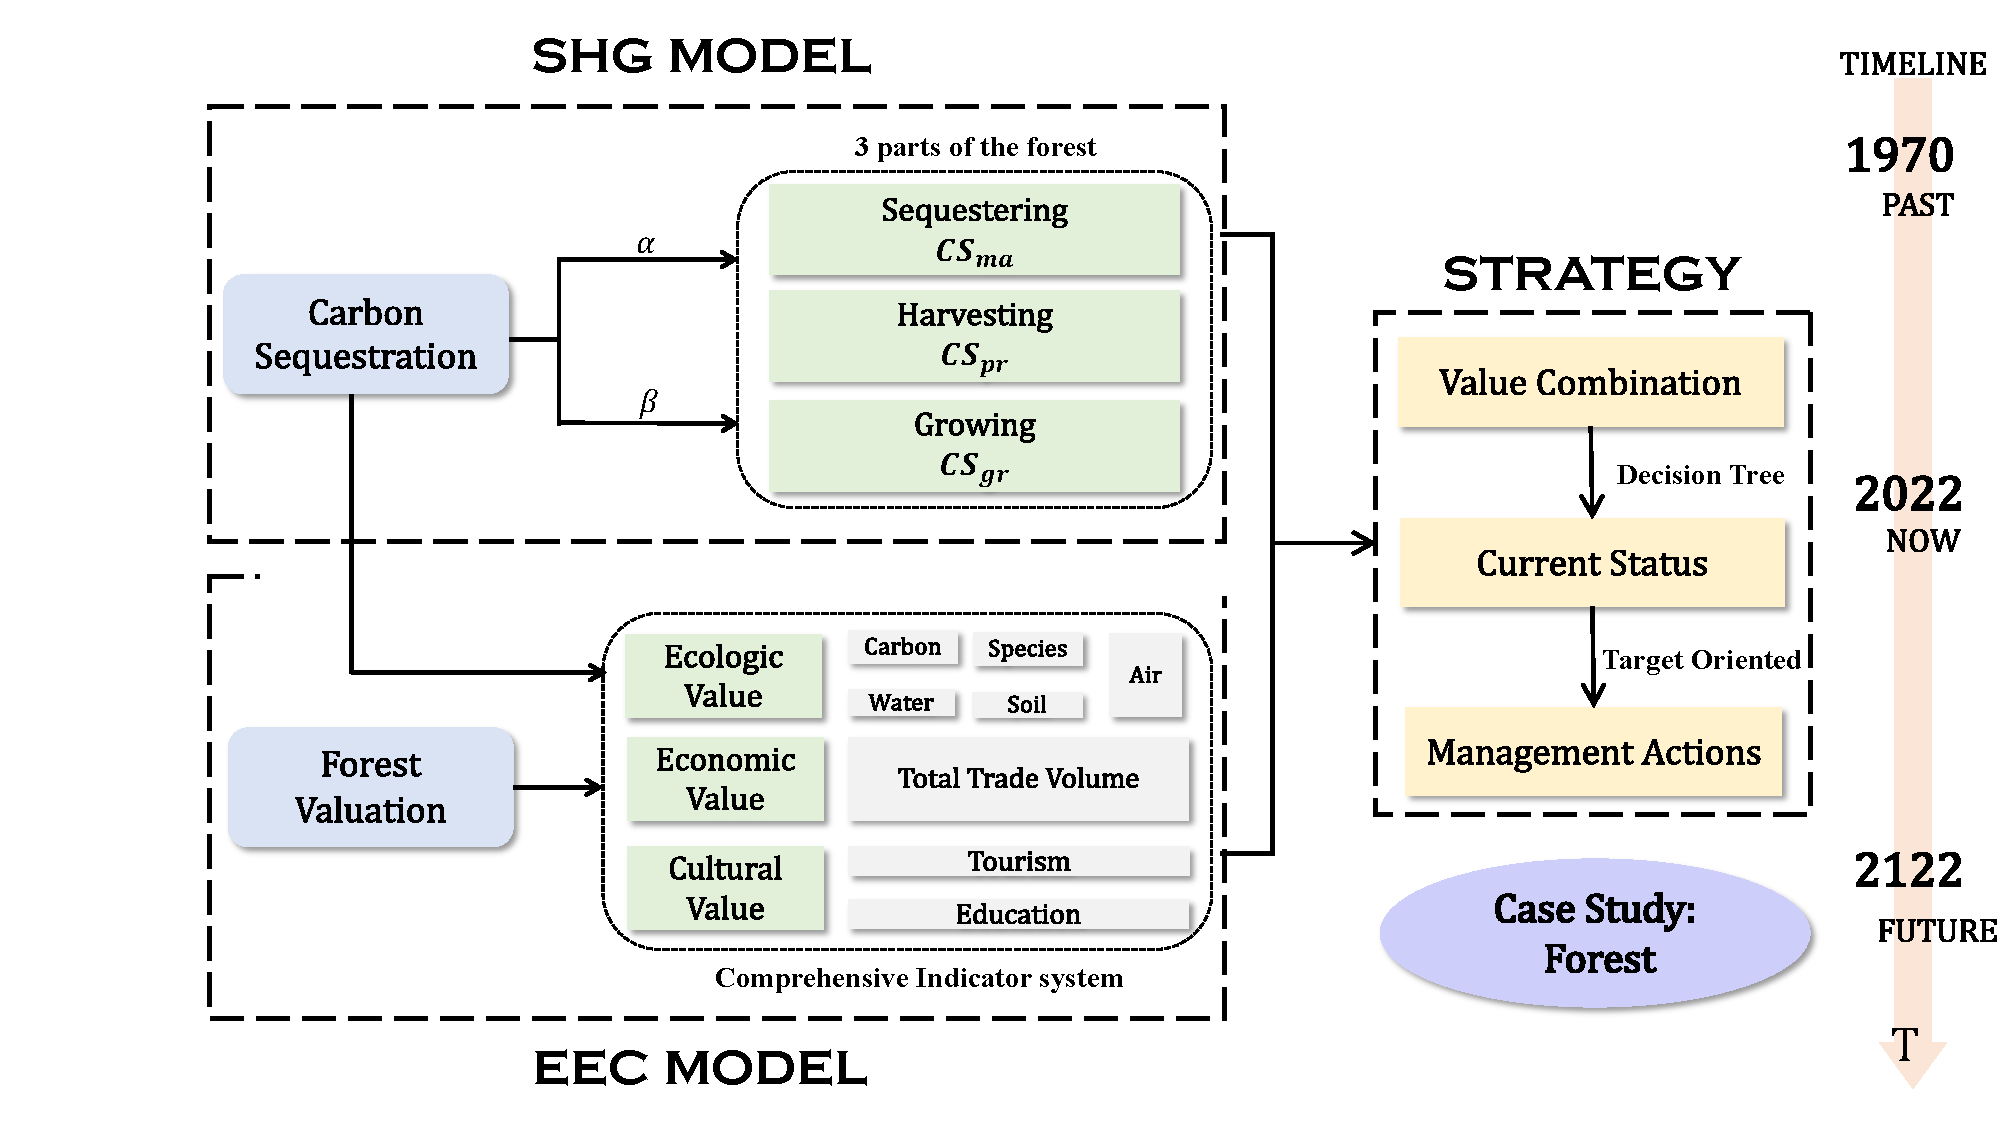
\includegraphics[width = 16.5cm]{mcmthesis-demo/figures/Our Work.pdf}
\caption{The whole framework of our essay}
\label{The whole framework}
\end{figure}